\subsection{Modelo estado de salud}
\label{modelo_health}

Representa el estado de salud de un dispositivo. La monitorización del estado de salud es una parte esencial del sistema ya que nos permitirá detectar comportamientos anómalos tales como una alta carga en CPU por un fallo seguramente en la programación, una carga anormal de memoria RAM, o detectar una temperatura de procesador demasiada alta para su correcto funcionamiento.
En la siguiente figura \ref{fig:modelo_iot_health_ecore} visualizamos el modelado en formato \gls{ecore} tree. En la figura anexa \ref{fig:modelo_iot_health_classes} podemos ver el modelo de clases.

\begin{figure}
	\centering
    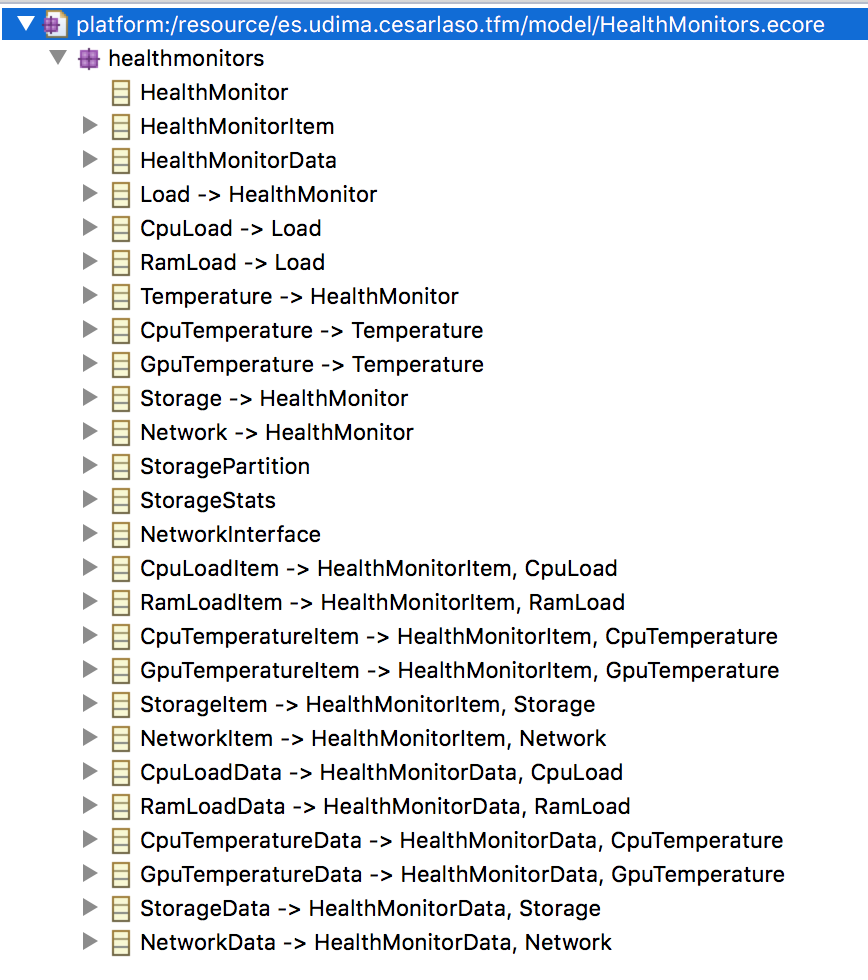
\includegraphics[scale=0.5]{images/emf_capturas/health_ecore.png}
    \captionmodelotree{Health}
    \label{fig:modelo_iot_health_ecore}
\end{figure}

Esta monitorización estará disponible en aquellos dispositivos que funcionen mediante un sistema operativo completo como Linux. Por este motivo, la comprobación del estado de salud no podrá ser aplicada a los dispositivos de tipo microcontrolador ya que al carecer de un sistema operativo completo, correr directamente en el hardware, o correr en un sistema operativo de tiempo real muy limitado no es posible en esta fase actual del desarrollo realizar esta implementación. En líneas futuras podríamos implementar dicha funcionalidad en el sistema operativo FreeRTOS \cite{freertos}, sistema operativo el cual corre el dispositivo ESP8266 \cite{esp8266}.

Este modelo será utilizado por el modelo de comunicación en la sección \ref{modelo_communication_health_services}.
